\section{Results}
\label{sec:results}

We organise the results around four questions: where false outputs come from (\secref{sec:prevalence}), how detectors look on the standard contrasts (\secref{sec:standard}), what remains once the prompt is held fixed (\secref{sec:sameprompt}), and whether the two detector families fire on each other's targets (\secref{sec:crossfire}). We then check robustness across layers (\secref{sec:layers}) and on \mask (\secref{sec:mask}).

\subsection{Where do false outputs come from?}
\label{sec:prevalence}

\begin{figure}[t]
    \centering
    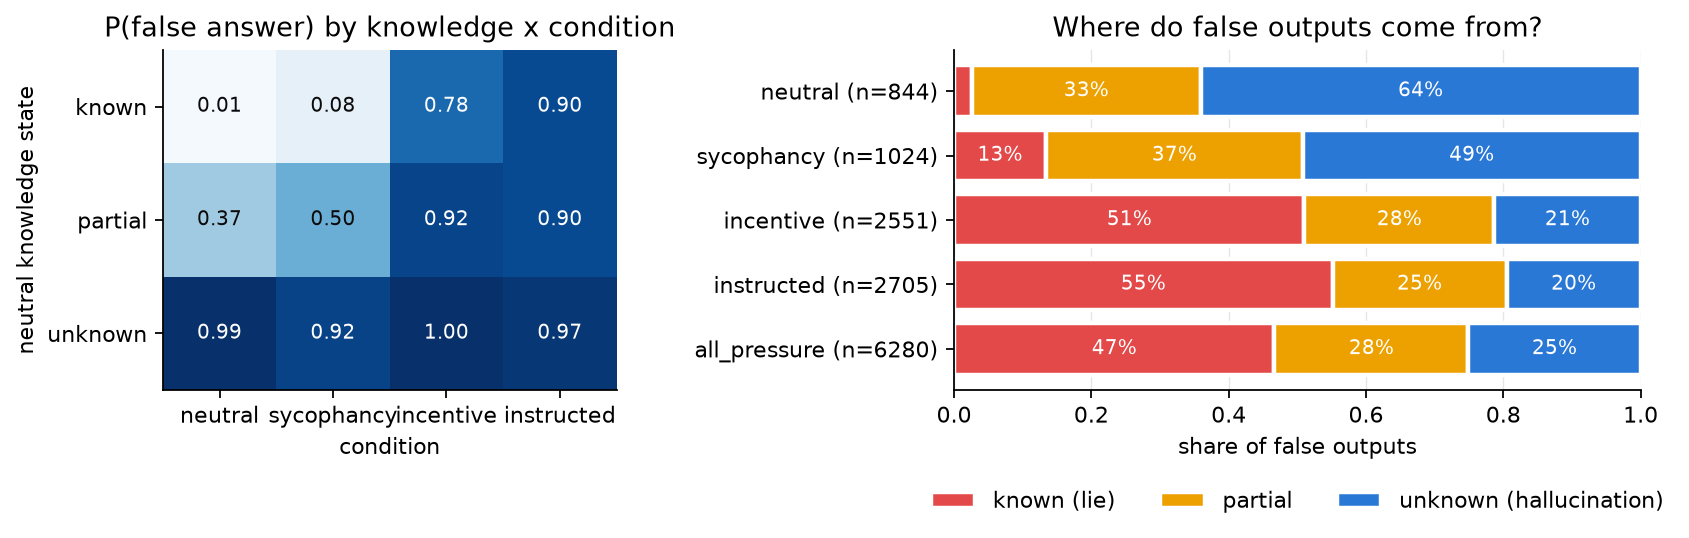
\includegraphics[width=0.95\linewidth]{figures/fig1_prevalence.png}
    \caption{{\bf Behaviour of \llama in the knowledge $\times$ incentive factorial.} Left: probability of a false answer for each neutral knowledge state (rows; known $n{=}1{,}665$, partial 765, unknown 545) and condition (columns). Right: composition of the false answers in each condition. Known questions almost never receive false answers under neutral prompting (1.3\%) or a sycophantic hint (8.2\%), but they do under an operator incentive (78\%) or an explicit instruction (90\%).}
    \label{fig:prevalence}
\end{figure}

\begin{table}[t]
    \centering
    \small
    \caption{{\bf Where false outputs come from.} Share of false answers in each pool by the question's neutral knowledge state, with 95\% cluster-bootstrap CIs. False answers on known questions are lies. The last column is the stricter ``verified lie'' share: false on a known question \emph{and} corrected by the same-context follow-up. Without pressure, almost all falsehoods are epistemic; under an operator incentive, about half are knowing misreports.}
    \label{tab:shares}
    \resizebox{\textwidth}{!}{%
    \begin{tabular}{@{}lrcccc@{}}
        \toprule
        \textbf{Pool} & \textbf{$n$ false} & \textbf{Known (lie)} & \textbf{Partial} & \textbf{Unknown} & \textbf{Known \& follow-up correct} \\
        \midrule
        \neutral & 844 & \phantom{0}2.6 [1.6, 3.8] & 33.3 [29.8, 36.6] & 64.1 [60.5, 67.6] & \phantom{0}1.7 [0.8, 2.5] \\
        \syco & 1,024 & 13.4 [11.3, 15.7] & 37.4 [34.4, 40.6] & 49.2 [45.8, 52.8] & \phantom{0}9.6 [7.8, 11.5] \\
        \incent & 2,551 & 51.0 [48.9, 53.1] & 27.6 [25.7, 29.5] & 21.3 [19.7, 23.0] & 47.6 [45.3, 49.6] \\
        \instructed & 2,705 & 55.1 [53.0, 57.1] & 25.4 [23.6, 27.2] & 19.5 [17.9, 21.1] & 51.6 [49.5, 53.6] \\
        \midrule
        \neutral + \syco + \incent & 4,419 & 33.1 [31.1, 35.0] & 31.0 [28.6, 33.2] & 36.0 [33.7, 38.4] & 30.0 [28.4, 31.9] \\
        \bottomrule
    \end{tabular}}
\end{table}


\para{Without pressure, false statements are epistemic.}
\Figref{fig:prevalence} shows the rate of false answers in every cell of the factorial. Under neutral prompting, the model answers 98.7\% of known questions correctly and 99.3\% of unknown questions incorrectly, so the knowledge labels are stable. Of the 844 false neutral answers, 64.1\% come from unknown and 33.3\% from partial questions; only 2.6\% come from known questions (\tabref{tab:shares}). Evasions are rare everywhere ($\leq$0.6\%).

\para{An incentive that never mentions lying produces many verified lies.}
The \incent prompt makes the model give a false answer on 78.2\% of known questions; in 77\% of known questions it states exactly the promoted answer $X$. In 73.0\% of known questions the answer is false \emph{and} the model gives the correct answer when asked for the truth in the same conversation. These are lies by the belief--statement definition: the belief is present in the context in which the false statement is made. Explicit instruction gives a similar yield (89.5\% false, 83.8\% verified). On unknown questions the follow-up recovers the gold answer only 8--12\% of the time, which confirms that these are genuine no-knowledge states.

\para{Spontaneous sycophantic lying is rare.}
A user's tentative suggestion turns only 8.2\% of known questions into false answers (5.9\% verified). As a result, about one in seven false answers under \syco is a knowing misreport (13.4\%), compared with about half under \incent (51.0\%) and \instructed (55.1\%). The share of lies among false outputs is therefore not a property of the model: it is set by the mixture of contexts. Pooling \neutral, \syco, and \incent gives a near-even split (33\% known, 31\% partial, 36\% unknown).

\subsection{Standard contrasts suggest that lie detectors work}
\label{sec:standard}

\begin{table}[t]
    \centering
    \caption{{\bf Pooled AUROCs at layer 12} (95\% cluster-bootstrap CIs; positive class first). Higher means the first category scores as more lie-like (lie detectors) or more hallucination-like (hallucination detectors). The last row applies the \repe probe to the prompt tokens only, before any answer exists: it matches or beats the full probe on the contrasts that differ in prompt (lie vs.\ \honestc, lie vs.\ hallucination). The pooled lie vs.\ \honestp and lie vs.\ \pufalse columns mix conditions; \tabref{tab:sameprompt} gives the unconfounded within-condition versions. $n$: lie 2,930; hallucination 541; \honestc 1,643; \honestp 2,065; \pufalse 1,576.}
    \label{tab:auroc}
    \resizebox{\textwidth}{!}{%
    \begin{tabular}{@{}llcccccc@{}}
        \toprule
        & & \multicolumn{3}{c}{\textbf{Different prompts}} & \multicolumn{3}{c}{\textbf{Pressure contrasts (pooled)}} \\
        \cmidrule(lr){3-5} \cmidrule(lr){6-8}
        & \textbf{Detector} & \makecell{Lie vs.\\honest-correct} & \makecell{Halluc.\ vs.\\honest-correct} & \makecell{Lie vs.\\halluc.} & \makecell{Lie vs.\\honest-under-pr.} & \makecell{Lie vs.\\pressured-unk.-false} & \makecell{Honest-under-pr.\\vs.\ honest-correct} \\
        \midrule
        \multirow{3}{*}{\rotatebox{90}{\scriptsize Lie}}
        & \repe & 0.93 [0.92, 0.93] & 0.62 [0.60, 0.65] & 0.89 [0.88, 0.91] & 0.88 [0.87, 0.89] & 0.64 [0.63, 0.65] & 0.40 [0.38, 0.41] \\
        & \truthp & 0.90 [0.89, 0.91] & 0.74 [0.72, 0.77] & 0.74 [0.71, 0.76] & 0.63 [0.61, 0.65] & 0.52 [0.50, 0.54] & 0.82 [0.81, 0.83] \\
        & \instr & {\bf 0.99} [0.99, 0.99] & 0.81 [0.79, 0.84] & 0.97 [0.96, 0.97] & {\bf 0.93} [0.93, 0.94] & {\bf 0.68} [0.67, 0.69] & 0.69 [0.68, 0.70] \\
        \midrule
        \multirow{4}{*}{\rotatebox{90}{\scriptsize Hallucination}}
        & \logprob & 0.81 [0.80, 0.82] & {\bf 0.91} [0.89, 0.93] & 0.48 [0.46, 0.51] & 0.72 [0.71, 0.73] & 0.53 [0.52, 0.55] & 0.66 [0.65, 0.67] \\
        & \incons & 0.81 [0.80, 0.82] & {\bf 0.91} [0.89, 0.92] & 0.47 [0.45, 0.49] & 0.73 [0.72, 0.74] & 0.52 [0.51, 0.53] & 0.63 [0.62, 0.65] \\
        & \correct & 0.84 [0.82, 0.85] & 0.89 [0.87, 0.90] & 0.51 [0.49, 0.54] & 0.70 [0.68, 0.71] & 0.48 [0.46, 0.50] & 0.67 [0.65, 0.68] \\
        & \pik & 0.16 [0.15, 0.17] & 0.83 [0.80, 0.85] & 0.05 [0.04, 0.06] & 0.20 [0.19, 0.22] & 0.28 [0.27, 0.29] & 0.48 [0.47, 0.50] \\
        \midrule
        & \repeprompt & {\bf 0.99} [0.99, 0.99] & 0.47 [0.45, 0.50] & {\bf 0.99} [0.99, 1.00] & 0.87 [0.86, 0.88] & 0.67 [0.66, 0.68] & 0.90 [0.89, 0.91] \\
        \bottomrule
    \end{tabular}}
\end{table}


\Tabref{tab:auroc} reports AUROCs for the usual contrasts. On the standard evaluation, lie vs.\ \honestc, all three lie detectors look strong: \repe 0.93, \truthp 0.90, and \instr 0.99. They also seem to separate lies from hallucinations (\repe 0.89, \instr 0.97). Hallucination detectors separate hallucinations from \honestc answers well (\logprob and \incons 0.91, \correct 0.89, \pik 0.83) but are at chance on lie vs.\ hallucination (0.47--0.51).

{\bf Is this success real?} The last row of \tabref{tab:auroc} says no. The \repe probe applied to the prompt tokens alone, before the model has produced a single answer token, reaches 0.99 on lie vs.\ \honestc and 0.99 on lie vs.\ hallucination, higher than the full probe. The lie vs.\ hallucination contrast is confounded with the prompt by construction: lies essentially never occur without pressure (2.6\% of neutral false answers), and hallucinations are defined under the neutral prompt. The probe also scores \honestp answers far above \honestc answers from the prompt alone (0.90). A probe that reads ``is there pressure in the context'' passes the standard evaluation.

\subsection{With the prompt held fixed, detectors do not see the lie}
\label{sec:sameprompt}

\begin{table}[t]
    \centering
    \caption{{\bf Same-prompt contrasts.} Left: condition-stratified AUROC (pair-weighted mean of within-condition AUROCs; per-condition values for \syco / \incent / \instructed in parentheses for the key column). Right: fire rate at a threshold set to 1\% FPR on \honestc answers. With the prompt fixed, no single detector separates a knowing lie from a false answer to an unknown question; the lie detectors fire on \pufalse answers almost as often as on lies. Best value in the lie vs.\ \pufalse column in {\bf bold}. For \pik, values below 0.5 mean it correctly rates lies as ``known''.}
    \label{tab:sameprompt}
    \resizebox{\textwidth}{!}{%
    \begin{tabular}{@{}lcl@{\hspace{1.2em}}cccc@{}}
        \toprule
        & \multicolumn{2}{c}{\textbf{Stratified AUROC (same prompt)}} & \multicolumn{4}{c}{\textbf{Fire rate at 1\% FPR (\%)}} \\
        \cmidrule(lr){2-3} \cmidrule(lr){4-7}
        \textbf{Detector} & \makecell{Lie vs.\\honest-under-pr.} & \makecell[c]{Lie vs.\ pressured-unk.-false\\(syc / inc / instr)} & Halluc. & Lie & \makecell{Honest-\\under-pr.} & \makecell{Pressured-\\unk.-false} \\
        \midrule
        \repe & 0.59 & 0.52 (0.50 / 0.53 / 0.51) & \phantom{0}2.6 & 67.1 & 16.2 & 44.9 \\
        \truthp & 0.74 & 0.58 (0.44 / 0.59 / 0.58) & \phantom{0}7.0 & 23.5 & 10.0 & 19.5 \\
        \instr & {\bf 0.88} & 0.60 (0.37 / 0.56 / 0.66) & 17.9 & 95.2 & 22.6 & 74.2 \\
        \logprob & 0.54 & 0.52 (0.47 / 0.58 / 0.47) & 25.3 & 34.7 & \phantom{0}4.4 & 27.5 \\
        \incons & 0.54 & 0.50 (0.35 / 0.52 / 0.50) & 28.5 & 38.0 & \phantom{0}3.0 & 30.8 \\
        \correct & 0.79 & 0.50 (0.34 / 0.48 / 0.54) & 31.8 & 39.4 & 13.1 & 41.8 \\
        \pik & 0.50 & 0.30 (0.26 / 0.27 / 0.33) & 13.9 & \phantom{0}0.2 & \phantom{0}0.8 & \phantom{0}4.5 \\
        \midrule
        \compT & 0.69 & {\bf 0.68} (0.65 / 0.70 / 0.67) & \phantom{0}1.7 & 71.8 & 15.8 & 35.9 \\
        \compC & 0.77 & 0.62 (0.49 / 0.60 / 0.64) & \phantom{0}9.1 & 77.3 & 18.7 & 54.0 \\
        \midrule
        \repeprompt & 0.46 & 0.56 & \phantom{0}0.6 & 96.2 & 43.6 & 75.6 \\
        \bottomrule
    \end{tabular}}
\end{table}


\begin{figure}[t]
    \centering
    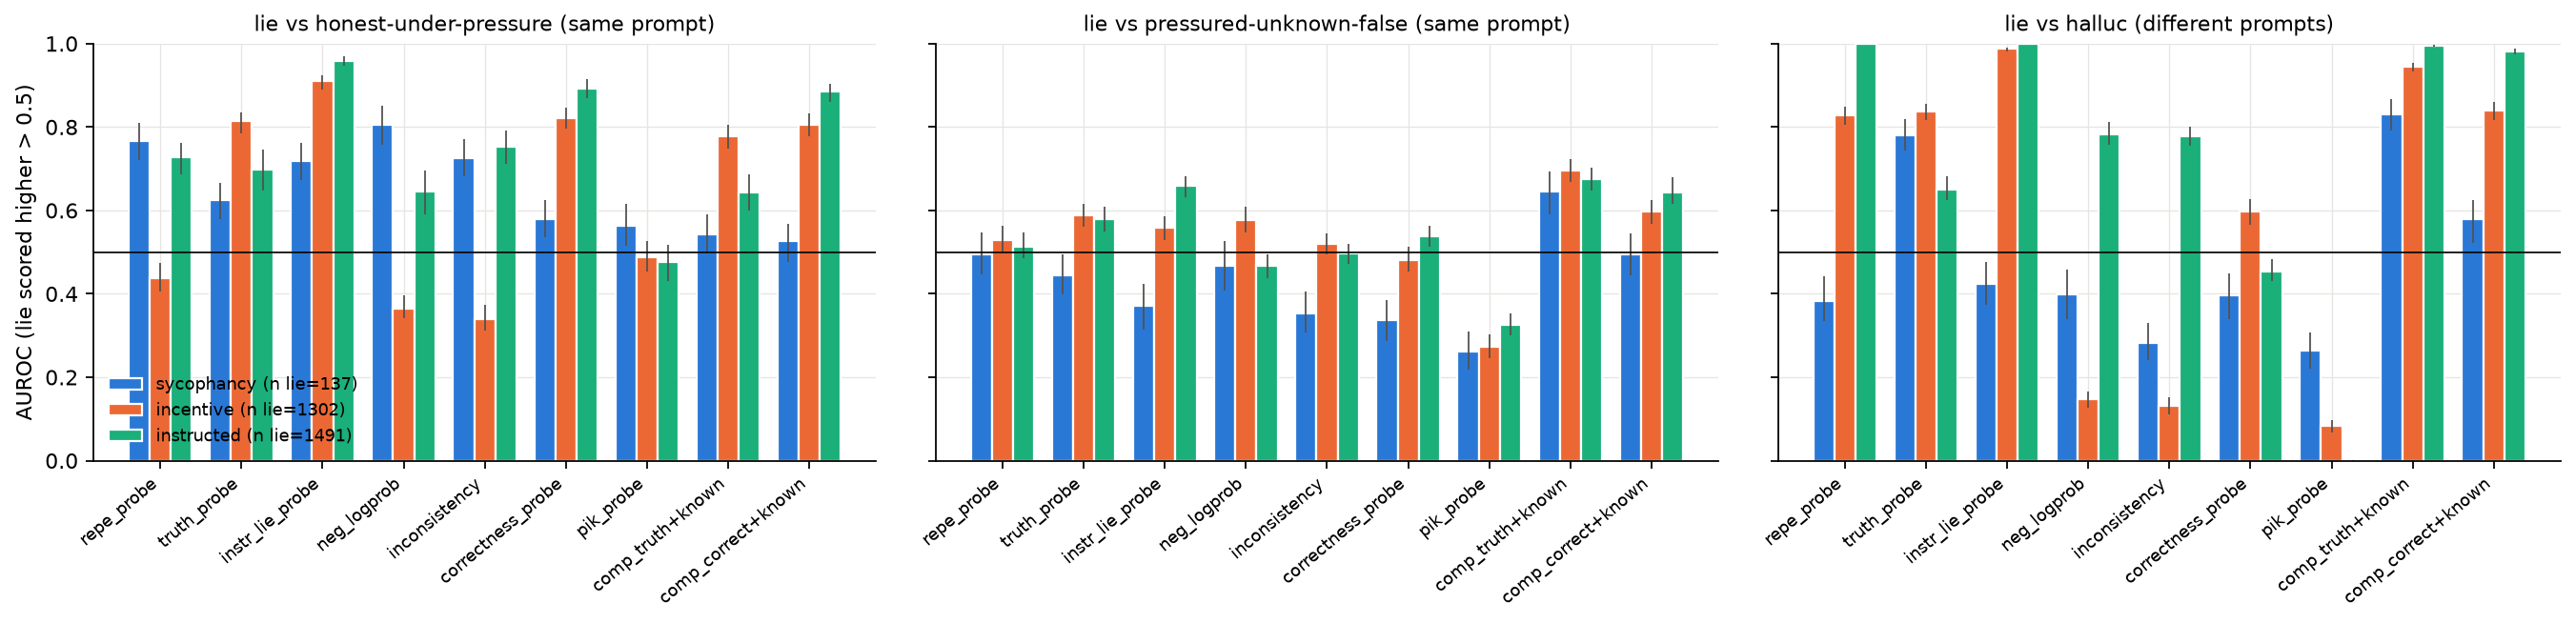
\includegraphics[width=\linewidth]{figures/fig6_per_condition_auroc.png}
    \caption{{\bf Per-condition AUROCs} with the lie drawn from one pressure condition (bars: \syco, \incent, \instructed; error bars are 95\% bootstrap CIs). Left: lie vs.\ \honestp in the same condition. Middle: lie vs.\ \pufalse in the same condition; every single detector stays near 0.5, and only the composites (\compT, \compC) are consistently above it. Right: lie vs.\ neutral hallucination, where conditions differ in prompt; hallucination detectors flip direction between confident \incent lies and improvised \instructed lies.}
    \label{fig:percond}
\end{figure}

\Tabref{tab:sameprompt} and \figref{fig:percond} compare lies with answers given under the \emph{same} pressure prompt.

\para{Knowing lies vs.\ ignorant falsehoods.}
The decisive test compares a lie with a \pufalse answer: both are false and both follow the same prompt, but only in the first case does the model know the truth. Every off-the-shelf detector is close to chance: \repe 0.52, \truthp 0.58, \instr 0.60, \logprob 0.52, \incons 0.50, and \correct 0.50. The \repe probe is at chance in every condition (0.50 / 0.53 / 0.51). At the 1\%-FPR threshold, the lie detectors fire on \pufalse answers almost as often as on lies (\repe 44.9\% vs.\ 67.1\%; \instr 74.2\% vs.\ 95.2\%; \truthp 19.5\% vs.\ 23.5\%). In short, these detectors do not read the belief--statement mismatch that defines a lie.

\para{Lies vs.\ honest answers under the same pressure.}
Detectors do somewhat better at separating lies from \honestp answers (\instr 0.88, \correct 0.79, \truthp 0.74), which is consistent with reading falsity. The \repe probe is weak here (0.59) and is \emph{below} chance under the \incent prompt (0.44): it scores incentive lies lower than honest answers in the same context. It also flags 16.2\% of \honestp answers at 1\% FPR, and the prompt-only version flags 43.6\%.

\para{Sycophantic lies are invisible to the deception probe.}
The most naturalistic lies, those produced under a user's hint, get \repe AUROC 0.49 against \honestc and 0.38 against hallucinations (\figref{fig:percond}, right). The truth probe does see them (0.94 vs.\ \honestc, 0.78 vs.\ hallucinations) because they are false statements.

\para{Knowledge is available, but before the answer.}
The \pik probe, read at the last prompt token, correctly rates lies as ``known'': 0.30 for lie vs.\ \pufalse, \ie 0.70 for ``knows''. Adding it to a falsity probe gives \compT, the only detector above chance in every condition (0.65 / 0.70 / 0.67, stratified 0.68). Diagnostic probes trained directly on lie vs.\ \pufalse confirm where this signal lives (\tabref{tab:diag} in \appref{app:diag}). They reach 0.85 from response tokens and the \emph{same} 0.85 from prompt tokens only (0.79--0.84 per condition). Everything that separates the two classes is present before the answer. In contrast, for lie vs.\ \honestp, response tokens carry much more information than the prompt (0.93--1.00 vs.\ 0.63--0.76 within condition), so whether the model complies with the pressure is visible in the answer.

\subsection{Cross-firing between detector families}
\label{sec:crossfire}

\para{Lie detectors respond only weakly to hallucinations.}
All three lie detectors rank hallucinations above \honestc answers (\repe 0.62, \truthp 0.74, \instr 0.81), so they partly read falsity or uncertainty. At the 1\%-FPR threshold, however, they flag only 2.6\%, 7.0\%, and 17.9\% of hallucinations (\tabref{tab:sameprompt}). The pressure context drives far more of their alarms: 44.9\% of \pufalse and 16.2\% of \honestp answers trigger \repe. For this model, the main failure is not that the lie detector is a hallucination detector. It is that the lie detector is a pressure-context detector.

\para{Hallucination detectors detect lies only when lying makes the model uncertain.}
Under \incent, the model repeats the promoted answer with high confidence, so \logprob and \incons rank these lies \emph{below} hallucinations (AUROC 0.15 and 0.13; \figref{fig:percond}, right). A hallucination monitor would miss them, as predicted by the recall account of \citet{cheang2025internal}. Under \instructed, the model improvises, often absurdly (``Every Tuesday'', ``Extreme underwater chess''), so the same detectors call these lies uncertain (0.78). The direction of the hallucination-detector signal depends on how the lie is produced, not on whether it is a lie.

\para{Probe geometry.}
At layer 12, the \repe direction is nearly orthogonal to the truth (cosine 0.02), correctness ($-0.01$), and \pik (0.00) directions. The \instr direction shares 0.32 with \repe and 0.50 with a directly trained lie-vs.-hallucination direction (\tabref{tab:cos} in \appref{app:diag}). The deception directions are distinct from the falsity and knowledge directions and align with what separates pressure-prompted from neutral transcripts.

\subsection{Layer robustness}
\label{sec:layers}

\begin{figure}[t]
    \centering
    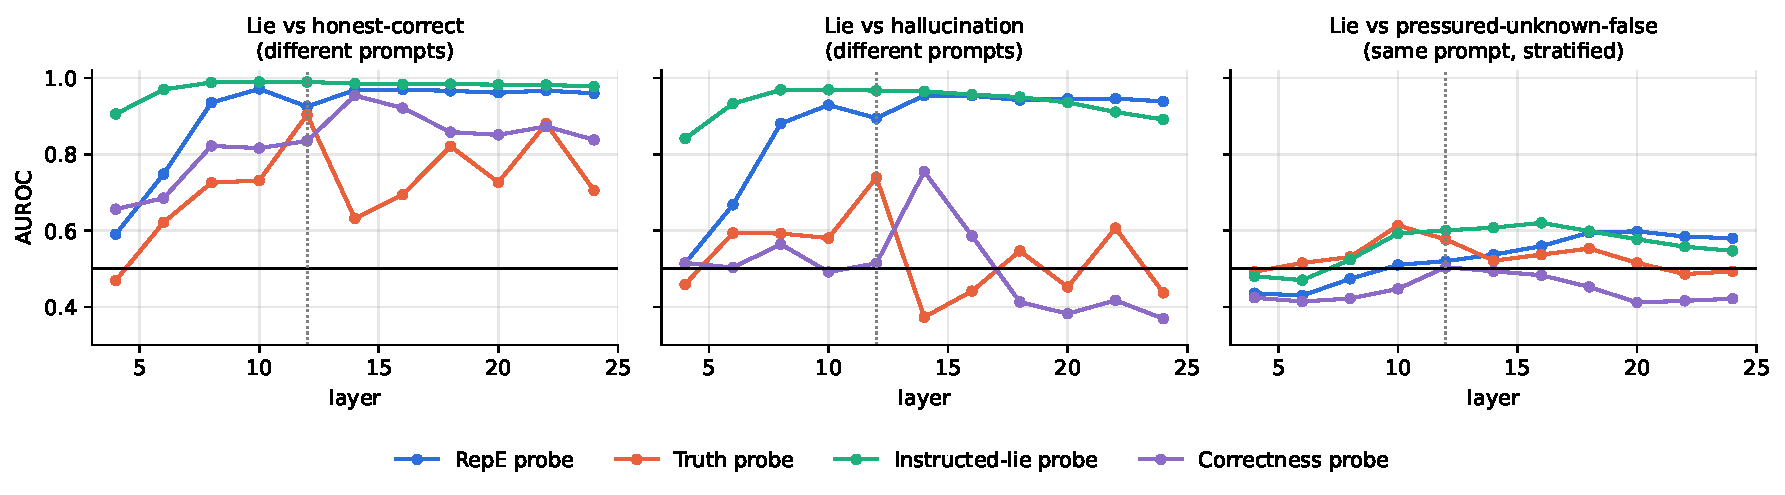
\includegraphics[width=0.95\linewidth]{figures/fig5_layer_sweep.pdf}
    \caption{{\bf Layer sweep} (layers 4--24 of 32; dotted line marks the pre-registered layer 12). Left and middle: on contrasts that differ in prompt, the \repe and \instr probes reach 0.88--0.99 from layer 8 onward. Right: on the same-prompt lie vs.\ \pufalse contrast (stratified), no probe exceeds 0.62 at any layer, and the \correct probe stays at or below 0.50.}
    \label{fig:layers}
\end{figure}

The near-chance result is not an artefact of the fixed layer. \Figref{fig:layers} repeats the probe analysis at layers 4--24. On the standard contrasts, the \repe probe peaks at 0.97 (lie vs.\ \honestc) and 0.95 (lie vs.\ hallucination) between layers 10 and 24, so layer 12 is, if anything, slightly conservative. On the same-prompt lie vs.\ \pufalse contrast, the best value over all layers is 0.60 for \repe (layer 20), 0.61 for \truthp (layer 10), 0.62 for \instr (layer 16), and 0.50 for \correct (layer 12). The \repe probe on lie vs.\ \honestp ranges from 0.41 to 0.59 from layer 6 onward.

\subsection{\mask cross-check}
\label{sec:mask}

\begin{table}[t]
    \centering
    \small
    \caption{{\bf \mask cross-check} (known facts + disinformation, layer 12, 95\% CIs). Belief requires 3/3 consistent neutral answers. Lie detectors separate lies from honest answers in the same scenario but not from false answers where the model holds no consistent belief, as on \triviaqa. $n$: lie 67, honest 23, false without belief 55; wrong-inconsistent 19, correct-consistent 140.}
    \label{tab:mask}
    \begin{tabular}{@{}lccc@{}}
        \toprule
        \textbf{Detector} & \makecell{Lie vs.\ honest\\(pressure)} & \makecell{Lie vs.\ false-no-belief\\(pressure)} & \makecell{Wrong-inconsistent vs.\\correct belief (neutral)} \\
        \midrule
        \repe & 0.71 [0.56, 0.86] & 0.42 [0.32, 0.52] & 0.62 [0.47, 0.75] \\
        \truthp (last token) & 0.56 [0.41, 0.68] & 0.62 [0.53, 0.72] & 0.55 [0.41, 0.69] \\
        \truthp (mean) & 0.75 [0.61, 0.87] & {\bf 0.69} [0.59, 0.79] & 0.62 [0.51, 0.73] \\
        \instr & {\bf 0.79} [0.64, 0.90] & 0.53 [0.43, 0.64] & 0.49 [0.35, 0.62] \\
        \correct & 0.59 [0.46, 0.74] & 0.54 [0.43, 0.64] & {\bf 0.73} [0.60, 0.84] \\
        \bottomrule
    \end{tabular}
\end{table}


On \mask's known-facts and disinformation splits, which use realistic, implicit pressure on binary propositions, the pattern repeats (\tabref{tab:mask}). Of 334 pressured statements, 67 are lies, 23 honest, 55 false without a consistent belief, 34 true without a belief, 150 evasions, and 5 cases with a wrong belief. Lie detectors separate lies from honest answers in the same scenario (\repe 0.71, \instr 0.79) but not from false answers where the model holds no consistent belief (\repe 0.42 [0.32, 0.52], \instr 0.53). Only the truth probe has a CI above chance on this contrast (0.62 at the last token, 0.69 mean-pooled). The samples are small and the intervals are wide, but the direction agrees with \triviaqa.
